%%%% Epidemic course interpretation
Moving onto the simulations, Figure \ref{fig:epidemic_course} shows the epidemic courses for the different networks where the top1\% to top12\% highest ranked nodes according to different centrality measures have been shut down (i.e. edges removal).
\begin{figure}[!h]
    \centering
    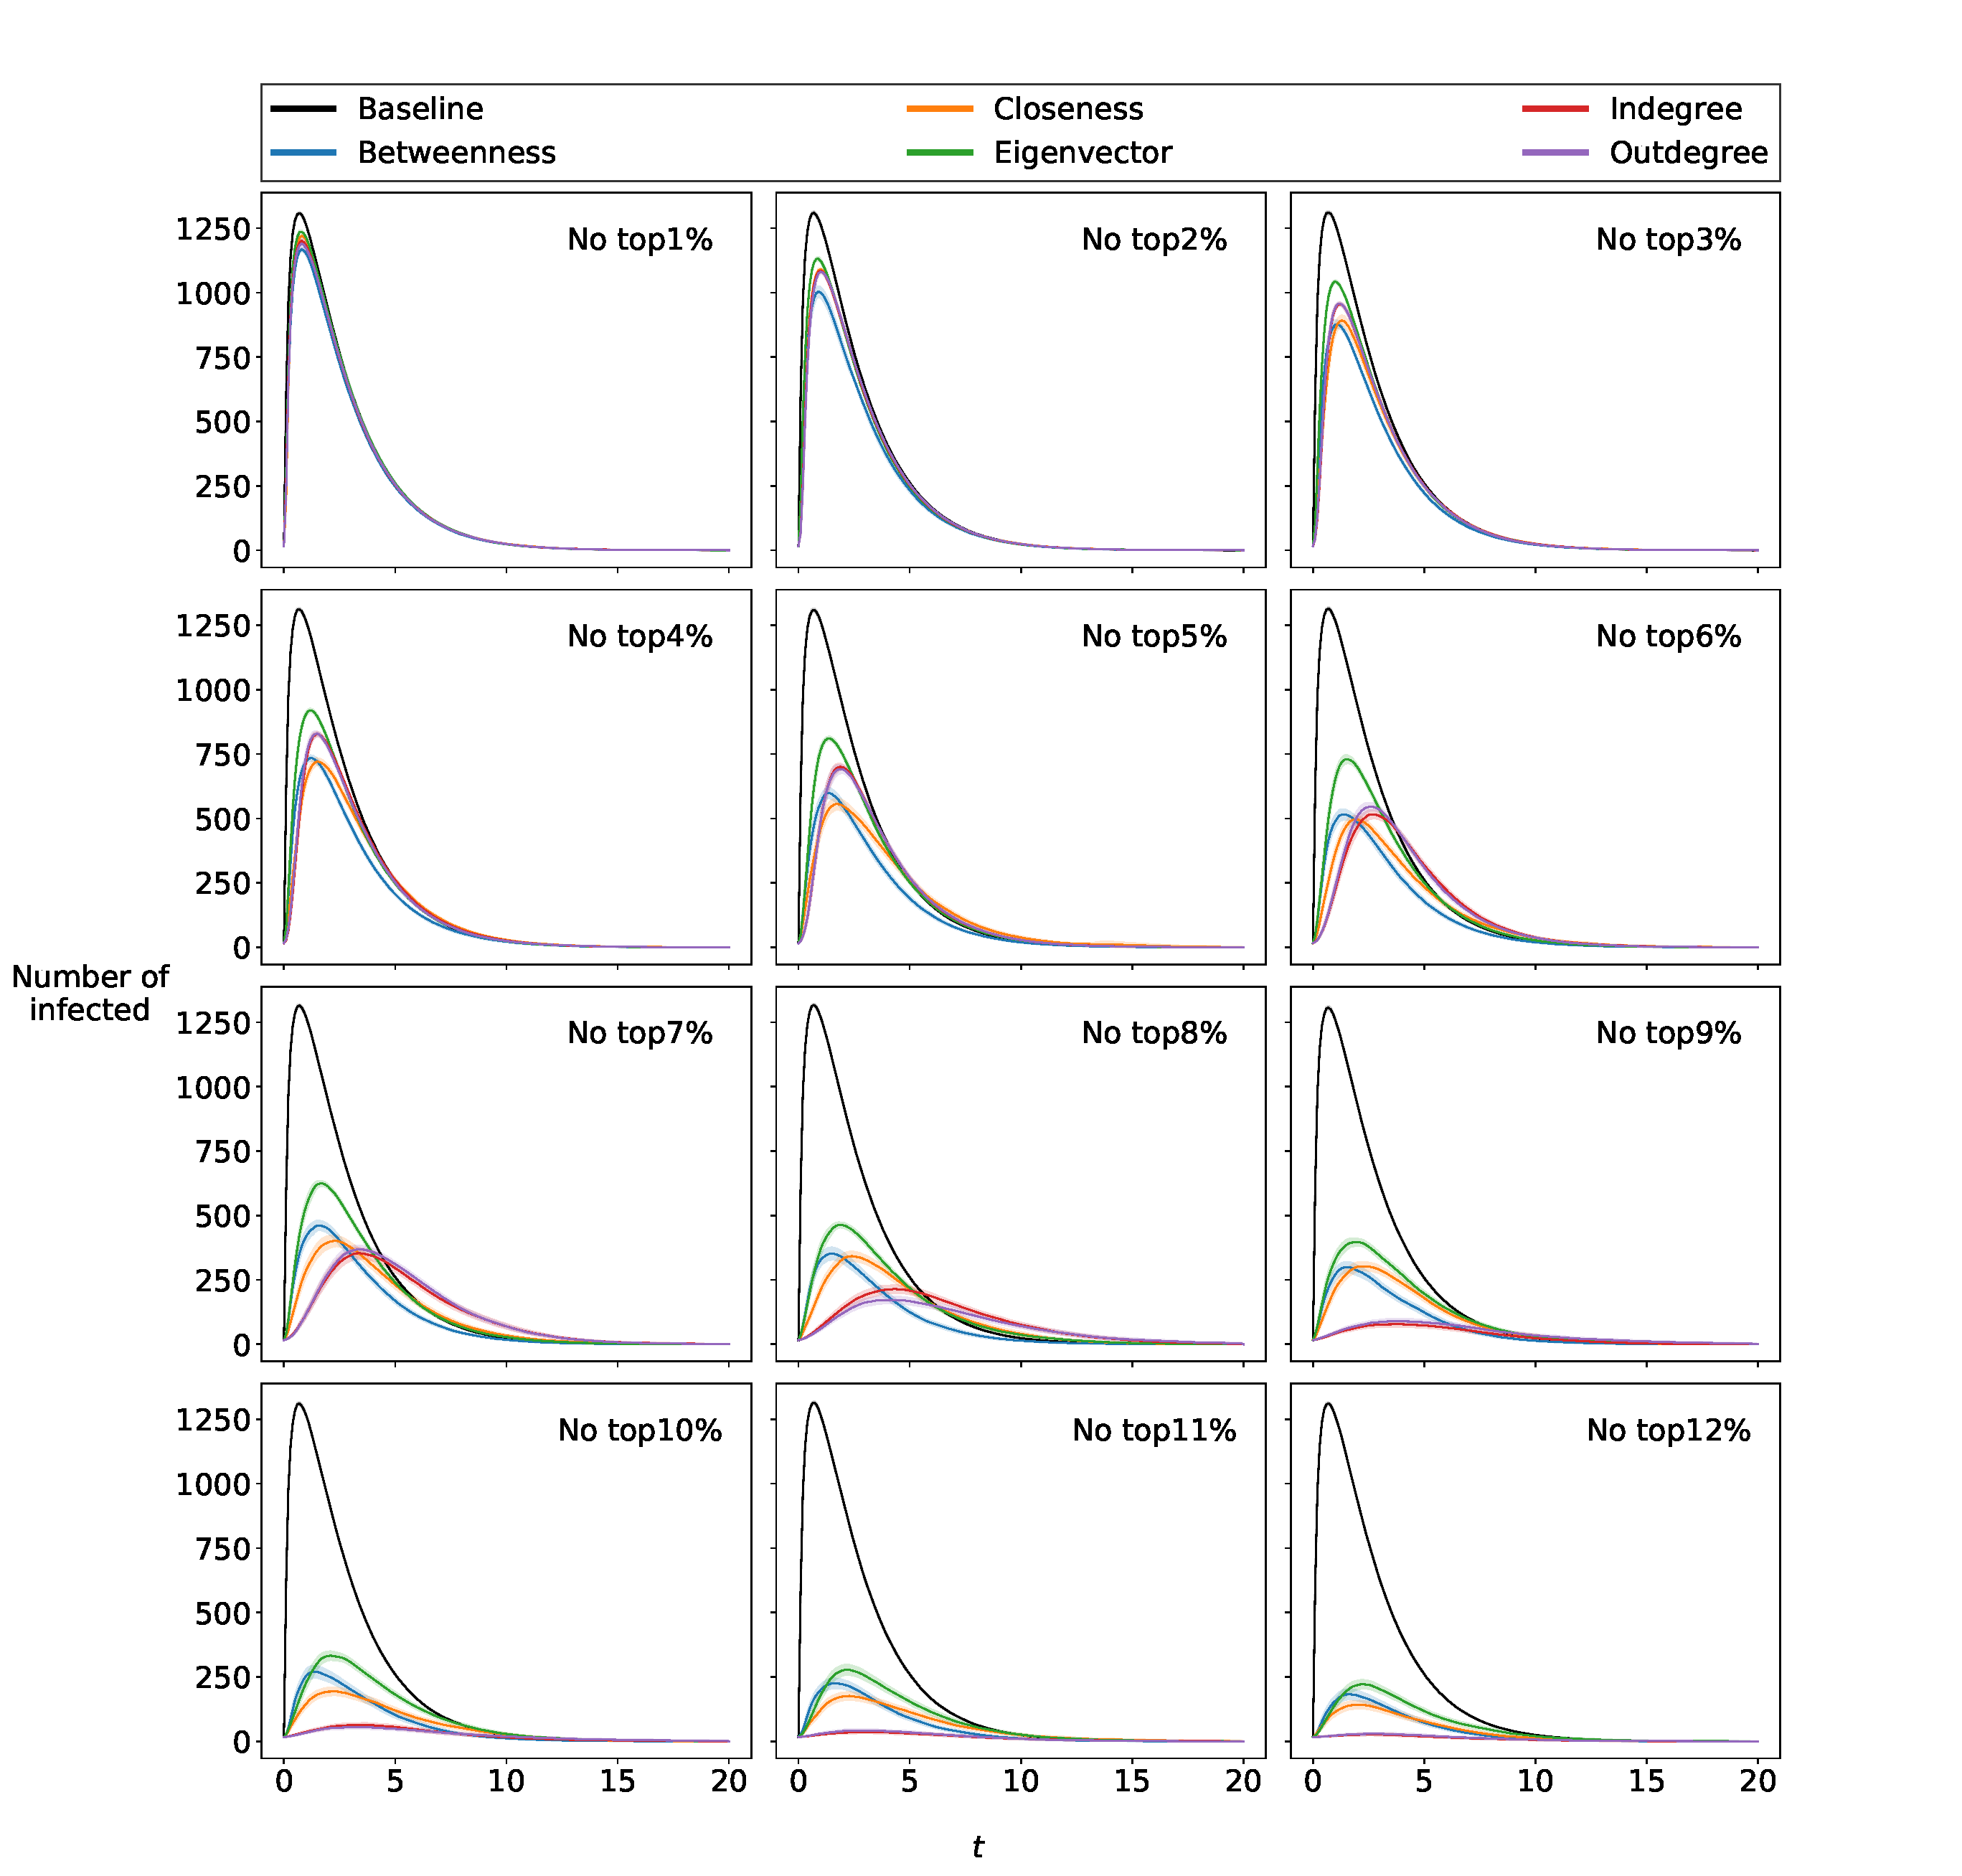
\includegraphics[width=\linewidth]{Figures/epidemic_course.pdf}
    \caption{Depicted are simulated epidemic courses across different scenarios. The (almost imperceptible) 95\%-confidence intervals can be seen as halo around all the lines.}
    \label{fig:epidemic_course}
\end{figure}
The baseline curves (in black) are always based on the full network and are thus nearly identical across the twelve panels, though minimal differences are always possible due to the finite nature of the simulation sample. We can observe two important features, one is the peak, i.e. the point with the highest number of infected nodes, and secondly the simulated evolution of infected nodes over time. A steep increase can be seen at the beginning, with infected cases shooting up to 1,250 within a short period of time, from where individual nodes start to recover and the curve slowly flattens out until it converges to zero after more than ten times the time (from $t$=20 on the value is fixed at 0). 

We can see that when only the top1\% key airports are closed, the course remains very similar to the baseline path, even though they represent a huge portion of the connections in relative terms due to the scale-free properties of our network. However, the more important airports are closed, the less sharply the number of infected airports shoots up and thus, the course of the epidemic proceeds more smoothly: the curves flatten. Notably, after a certain point (around 10\% of nodes closed) we can hardly notice any change in the evolution of the infection. This again originates from the fact, that our network has scale-free properties which further resumes in a power-law distribution of the evolution concerning the number of infections, such that after a certain point the nodes being closes are quite irrelevant.

It is also noticeable that from the extraction of the top 9\% IC and OC nodes (red and purple lines, respectively), the curves become nearly flat, with close to no increase, remaining at around zero. In contrast to the BC, CC and EC which still show peaks of infected cases, even though they get reduced by up to 80\%, until it barely changes after the removal of more than top 10\% nodes. Moreover, the slopes of the curves are much flatter, since the increase in infected cases is less sharp at the beginning and is decreasing slowly. To examine these three centrality measures in more depth, it can be seen that the slope of the curve is approximately the same for all of them at the beginning, with the peak being shallowest for CC and highest for EC. The fall of the infected cases is slower for the CC and more drastic for the EC and BC, whereby for the latter the recovery process occurs earlier and more strongly and undercuts the CC in this measure already early, despite the latter’s smaller peak.

